
\begin{figure}[t]
\setlength{\belowcaptionskip}{-10pt}
\setlength{\abovecaptionskip}{0pt}
\begin{minipage}[t]{0.49\linewidth}
  \centering 
  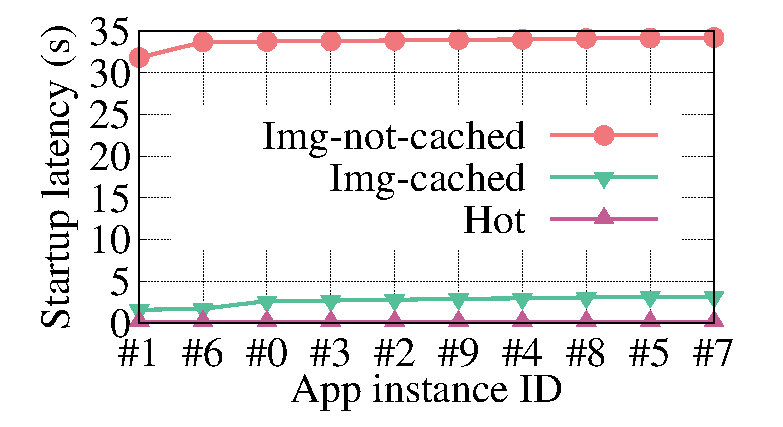
\includegraphics[width=1\linewidth]{figs-eval/case-scheduler-motiv.eps}
  \footnotesize    
\textbf{(a) Motivation (Knative)}
\end{minipage}  
\begin{minipage}[t]{0.49\linewidth}
  \centering 
  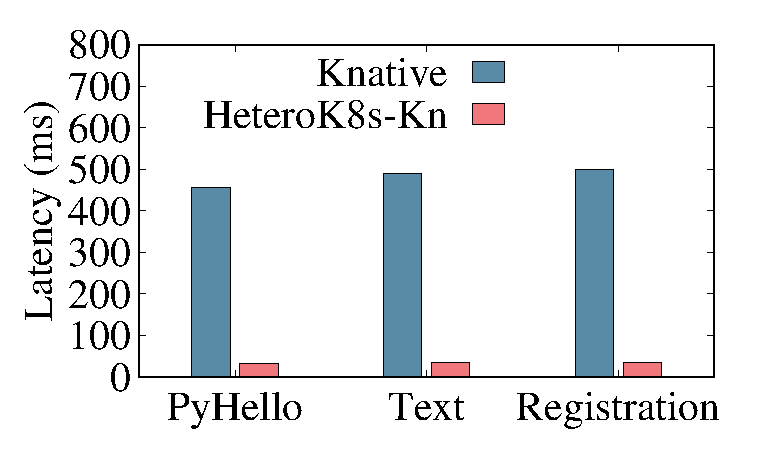
\includegraphics[width=1\linewidth]{figs-eval/case-scheduler-opt.eps}
  \footnotesize    
\textbf{(b) Optimization results}
\end{minipage}  
\caption{\textbf{Offloading scheduler for image-aware scheduling.}
  % \textit{MR for MapReduce. XPU for Cross-PU.}
  }
  \label{fig:eval-scheduler}
\end{figure}



\subsection{Case Study: Offloading Scheduler}
\label{s:case-scheduler}


\myparagraph{Motivation.}
Startup latency is one of the most important metrics for cloud-native apps~\cite{socc20-serverlessbench}.
Although there are many efforts to utilize C/R, fork, and caching, to optimize the container startup latency, we observe significant challenges from \emph{image pull},
i.e., if a request is scheduled to a node without the prepared image, the platform will pull the image first and then launch the instance.
To analyze the costs,
we evalaute the response latency in Knative~\cite{knative}, a widely-used FaaS system, with Kperf.
As shown in Fig.\ref{fig:eval-scheduler}-a, the latency of image not-cached is about 10x longer than the image-cached case.


\myparagraph{Idea and challenges.}
Cloud-native platforms usually rely on a global scheduler to schedule a Node for a request, e.g., kube-scheduler in K8s.
An idea is \emph{image-aware scheduler}, which prefers to assign a request to a Node with prepared images,
e.g., K8s supports image-locality policy~\cite{image-locality}.
However, this requires scheduler to maintain the image information of all nodes.
For a real-world environment, caching all image information requires 1GB--10GB resource.
Besides, updates of image status will notify the scheduler,
making it the bottleneck component in the control plane.

\myparagraph{Solution.}
\sys can offload the image cache in the scheduler to the DPU, utilizing the redundant resources to maintain images.
Moreover, as DPU is more closer to the network, it is more reasonable to use DPU to update image status.
Based on the offloading, we design an image and tempalte (for container fork~\cite{10.1145/3503222.3507732}) aware policy (as a kube-scheduler plugin), which will prioritize nodes with template instances and cached images.
We support Knative (w./o. modification) on \sys with the offloaded scheduler and new policy.
As shown in Fig.\ref{fig:eval-scheduler}-b, we analyze the avg latency in the whole cluster (four machines), and \sys-Kn can reduce the avg latency from 481ms to 33ms (14.4x).
